\documentclass[12pt]{article}
\usepackage[utf8]{inputenc}
\usepackage[a4paper, total={6.5in, 8.5in}]{geometry}
\usepackage{authblk}
\usepackage{multirow}
\usepackage{graphicx}
\usepackage{amsmath}
\usepackage{biblatex}
\usepackage{rotating}
\usepackage{ragged2e}
\usepackage{multicol}
\usepackage{float}
\usepackage{algpseudocode}
\usepackage{enumitem}
\usepackage{caption}
\usepackage{subcaption}
\usepackage{hyperref}
\hypersetup{
    colorlinks=true,
    linkcolor=blue,
    }
\usepackage[label=corner]{karnaugh-map}
\usepackage[siunitx, RPvoltages]{circuitikz}
\usetikzlibrary{calc}
\usepackage{tikz}
\usetikzlibrary{positioning}

\title{CSE 210 \\
Computer Architecture Sessional \\
\vspace{10mm}
Assignment-1: 4-bit ALU Simulation \\
\vspace{20mm}
Section - A2 \\
Group - 02 \\
\vspace{15mm}
\RaggedRight
Members of the Group: \\
\normalsize	{
\begin{enumerate}[label=\roman*]
    \item 2105043 - Monjur Hossain Khan
    \item 2105046 - Mohammad Raihan Rashid
    \item 2105047 - Himadri Gobinda Biswas
    \item 2105049 - Amit Saha
    \item 2105055 - Md. Abrar Jahin
\end{enumerate}
}
}
\author{}
\date{}

\begin{document}

\maketitle

\newpage

\section{\large{Introduction}} The \textbf{Arithmetic and Logic Unit (ALU)} serves as the computational core of a computer, responsible for performing essential mathematical and logical operations. It is fundamentally a \textbf{combinational digital circuit} that executes arithmetic and bitwise logical operations on integer binary numbers. Being a key component of computing hardware, the ALU is vital to both \textbf{Central Processing Units (CPUs)} and \textbf{Graphics Processing Units (GPUs)}.\ An ALU comprises two primary components: the \textbf{Arithmetic Unit} and the \textbf{Logic Unit}, which together handle a broad set of operations. These include arithmetic functions like addition, subtraction, incrementing, decrementing, and transferring, as well as logical functions such as \textbf{NOT}, \textbf{OR}, \textbf{XOR}, and \textbf{AND}. A \textbf{control unit} directs data from registers to the ALU's inputs, and \textbf{selection lines} or bits determine which operation to perform. In general, an ALU with \textit{$k$ selection lines} can handle \textit{$2^k$} distinct operations. For our implementation, the ALU is configured with \textit{three selection inputs}.\ The \textbf{parallel adder} forms the core of the arithmetic section of the ALU, enabling various arithmetic operations by utilizing \textbf{multiplexed inputs}. 

Logical operations, on the other hand, are carried out using specific \textbf{Integrated Circuits (ICs)}, although in optimized designs, an IC might perform operations beyond its intended use.\ In our design, we incorporate \textbf{four status flags} or outputs, labeled as \textbf{C (Carry Flag)}, \textbf{Z (Zero Flag)}, \textbf{V (Overflow Flag)}, and \textbf{S (Sign Flag)}. These flags convey the following:

\begin{description} \item[CF:] The \textbf{Carry Flag (CF)} reflects the \textit{$C_{out}$} of the ALU's adder. If a carry is generated, this flag is set to \textbf{1}; otherwise, it remains \textbf{0}. All logical operations result in a \textit{CF} value of \textbf{0}.

\item[ZF:] The \textbf{Zero Flag (ZF)} is set if the ALU's most recent operation yields a result of \textbf{0}; otherwise, it is cleared.

\item[VF:] The \textbf{Overflow Flag (VF)} is set when an arithmetic operation involving two positive numbers results in a negative outcome or when two negative numbers result in a positive outcome, indicating overflow. Logical operations reset this flag.\


\begin{equation}
    V = C_3 \oplus C_{out}\\
\end{equation}

Here, \textit{$C_3$} represents the carry generated during the addition of $A_2$, $B_2$ \& $C_2$, while \textit{$C_{out}$} is the output carry from the adder.

\item[SF:] The \textbf{Sign Flag (SF)} reflects the \textbf{most significant bit (MSB)} of the ALU's output. \end{description}


\newpage
\section{\large{Problem Specification with Assigned Instructions}}
Design a 4-bit ALU with three selection bits cs0, cs1 and cs2 for performing the following operations:
\begin{table}[H]
    \centering
    \begin{tabular}{||c|c|c|c|c||}
    \hline
         \multicolumn{3}{||c|}{Control Signals} & \multirow{2}{*}{Functions} & \multirow{2}{*}{Description}\\
         \cline{1-3}
         cs2 & cs1 & cs0 & & \\
         \hline
         \hline
         0 & 0 & 0 & Add & $A + B$ \\
         0 & X & 1 & Sub & $A - B$ \\
         0 & 1 & 0 & AND & $A \land B$\\
         1 & 0 & 0 & XOR & $A \oplus B$\\
         1 & X & 1 & Complement A & $\overline{A}$\\
         1 & 1 & 0 & NEG A & $-A$\\
         \hline
    \end{tabular}
    \caption{Problem Specification}
    \label{tab:Table1}
\end{table}
\vspace{15mm}

% \begin{figure}[H]
%     \centering
%     \includegraphics[width=0.8\textwidth]{alu_block_1.png}
%     \caption{4-bit ALU}
%     \label{fig:alu_block_1}
% \end{figure}

\begin{figure}[H]
\centering
\begin{tikzpicture}
    \node[draw, rectangle, minimum width=3.5cm, minimum height=2cm] (alu) at (0, 0){ALU};
    \draw[latex-] (alu.130) |- ++ (0, 1.5) node[above left=1.5cm and -1.35cm of alu] {cs2};
    \draw[latex-] (alu.90) |- ++ (0, 1.5) node[above left=1.5cm and -2.20cm of alu] {cs1};
    \draw[latex-] (alu.50) |- ++ (0, 1.5) node[above left=1.5cm and -3.10cm of alu] {cs0};
    \node at (-6, 0) {Input};
    \draw[latex-] (alu.165) -- ++ (-2, 0) node[pos=1.1] {A};
    \draw[latex-] (alu.195) -- ++ (-2, 0) node[pos=1.1] {B};
    \draw[-latex] (alu.east) -- ++ (2, 0) node[pos=1.45] {Output};
\end{tikzpicture}
    \vspace{5mm}
    \caption{4-bit ALU}
    \label{fig:alu_block_1}
\end{figure}



\newpage
\section{\large{Detailed Design Steps with K-maps}}

\subsection{Design Steps}
\begin{enumerate}
    \item The arithmetic logical unit computes 3 arithmetic operations (Add, Sub,  and, NEG A) and 3 logical operations(AND, XOR and, Complement A)  with the help of two 4-bit full adder and three multiplexer. 

    \item For the adder, the \textbf{first input $X_i$}  varies with different control bit input. It depends on \textbf{both $A_i$ and $B_i$}. There are 4 possible values of $X_i$: \textbf{$A_i$, $A \land B$, $A \oplus B$ and $\overline{A_i}$}. Thus, we had to use \textbf{\textit{two} dual 4$\times$1 MUX} for choosing the correct required value. We also generated $S_1$ (k-map: \ref{kmap:S_1}) and $S_2$ (k-map: \ref{kmap:S_2}) for selecting the proper value for the required operation. 

    \item The second input $Y_i$ also varies with different control bit input. These are as follows: \textbf{$B_i$, $\overline{B_i}$} and \textbf{0}. For the selection we used \textbf{\textit{one} quad 2$\times$1 MUX}. The selection between  $B_i$ and $\overline{B_i}$ is done using $S_3$ (k-map:\ref{kmap:S_3}). For generating \textbf{0} we used the another function for $en_3$ (k-map: \ref{kmap:en_3}).

    \item We also generated $C_{in}$ (k-map: \ref{kmap:Cin}), as the input of $C_{in}$  varies according the different required operations and it is kept \textbf{0} during logical operations.
    
    \item For the \textbf{Overflow Flag (VF)}, we needed both $C_3$ and $C_{out}$. Now, the tricky part was how to get the $C_3$ (since it is handled internally in the adder). We had a lot of design decision to make which are further discussed in the discussions. But we opted to using two adders. The first three bits of $X_i$ and $Y_i$ are added in the first adder. The the $S_3$ ($C_3$) from the first adder is given as $C_{in}$ to the second adder. Now we have a $C_3$ and we get the required $C_{out}$ from the $S_1$ terminal of the second adder. This, $C_{out}$ is also the \textbf{Carry Flag (CF)} of the adder.

    \item \textbf{Zero flag (ZF)} is computed by firstly ORing the two pairs of output bits respectively ( $S_0 \lor S_1 $ ) and ( $S_2 \lor S_3$ ). Then we pass the output into a NOR gate and finally get the ZF as output. 

    \item \textbf{The Sign Flag (SF)} is technically the MSB. So, we just take the output $S_0$ from the second adder as SF.

\end{enumerate}
\newpage
\subsection{K-maps}
We will be following Table \ref{tab:truth_table} to construct the K-maps for intermediate selection bits.
\subsubsection{K-map for $S_1$}
$S_1$ is the first selection bit for the dual 4$\times$1 Multiplexer that selects the first input of the adder. There are 4 possible values of $X_i$: \textbf{$A_i$, $A \land B$, $A \oplus B$ and $\overline{A_i}$}.\\
\begin{center}
\begin{karnaugh-map}[4][2][1][$cs0$][$cs1$][$cs2$]
    \maxterms{0, 1, 3, 4}
    \minterms{2, 5, 6, 7}
    \implicant{5}{7}
    \implicant{2}{6}
    \label{kmap:S_1}
\end{karnaugh-map}
\end{center}
So, there are four minterms. We use basic operations (AND, OR, NOT, NOR) IC to implement it. 
\[ S_1 =  cs2 \cdot cs0 + cs1 \cdot \overline{cs0}  \]

\subsubsection{K-map for $S_2$}
$S_2$ is the second selection bit for the dual 4$\times$1 Multiplexer that selects the first input of the adder.\\
\begin{center}
\begin{karnaugh-map}[4][2][1][$cs0$][$cs1$][$cs2$]
    \minterms{4, 5, 6, 7}
    \maxterms{0, 1, 2, 3}
    
    \implicant{4}{6} % This will mark all minterms in a single implicant
    \label{kmap:S_2}    
\end{karnaugh-map}
\end{center}
$S_2$ is simply $cs2$.
\[S_2 = cs2 \]

\subsubsection{K-map for $S_3$}
$S_3$ is the selection bit for $Y_i$. The possible valued determined by $S_3$ are as follows: \textbf{$B_i$ \text{, and} $\overline{B_i}$}.
\begin{center}
\begin{karnaugh-map}[4][2][1][$cs0$][$cs1$][$cs2$]
    \minterms{1, 3}
    \maxterms{0}
    \terms{2, 4, 5, 6, 7}{X}
    \implicant{1}{7} % This will mark all minterms in a single implicant
    \label{kmap:S_3}
\end{karnaugh-map}
\end{center}

$S_3$ is simply $cs0$
\[S_3 = cs0\]

\subsubsection{K-map for $C_{in}$}
It is the input carry bit of the adder. It will be $1$ at the time of \textit{Sub and NEG A} operation. 
\begin{center}
\begin{karnaugh-map}[4][2][1][$cs0$][$cs1$][$cs2$]
    \minterms{1, 3, 6}
    \maxterms{0, 2, 4, 5, 7}
    \implicant{6}{6}
    \implicant{1}{3}
    \label{kmap:Cin}
    
\end{karnaugh-map}
\end{center}
\[C_{in} =  \overline{cs2} \cdot cs0 + cs2 \cdot cs1 \cdot \overline{cs0}\]

\subsubsection{K-map for $en_3$}
$en_3$ for the second multiplexer is used for making all the bits of $Y_i$ \textbf{0}. In all operations enable is high(resulting $Y_i$ being \textbf{0}), except for add and sub operation. 
\begin{center}
\begin{karnaugh-map}[4][2][1][$cs0$][$cs1$][$cs2$]
    \minterms{2, 4, 5, 6, 7}
    \maxterms{0, 1, 3}
    \implicant{2}{6}
    \implicant{4}{6}
    \label{kmap:en_3}
\end{karnaugh-map}
\end{center}
The equation of $en_3$ is as follows:
\[c = cs2 + cs1 \cdot \overline{cs0}\]

\newpage
\section{\large{Truth Table}}
For better interpretation of the variables used, refer to Figure \ref{fig:block_diagram}.
\begin{table}[H]
    \centering
    \begin{tabular}{|ccc|c|c|c|c|c|c|c|c|}
    \hline
         cs2 & cs1 & cs0 & Function & $X_i$ & $S_2$ & $S_1$ & $Y_i$ & $S_3$ & $en_3$ & $C_{in}$  \\
         \hline
         0 & 0 & 0 & Add & $A_i$ & 0 & 0 & $B_i$ & 0 & 0 & 0  \\
         0 & 0 & 1 & Sub  & $A_i$ & 0 & 0 & $\overline{B_i}$ & 1 & 0 & 1 \\
         0 & 1 & 0 & AND & $A_i \land B_i$ & 0 & 1 & 0 & X & 1 & 0 \\
         0 & 1 & 1 & Sub  & $A_i$ & 0 & 0 & $\overline{B_i}$ & 1 & 0 & 1 \\
         1 & 0 & 0 & XOR & $A_i \oplus B_i$ & 1 & 0 & 0 & X & 1 & 0 \\
         1 & 0 & 1 & Complement A & $\overline{A_i}$ & 1 & 1 & 0 & X & 1 & 0 \\
         1 & 1 & 0 & NEG A & $\overline{A_i}$ & 1 & 1 & 0 & X & 1 & 1 \\
         1 & 1 & 1 & Complement A & $\overline{A_i}$ & 1 & 1 & 0 & X & 1 & 0 \\
         \hline
    \end{tabular}
    \caption{Truth Table for Intermediate I/0}
    \label{tab:truth_table}
\end{table}


\newpage
\section{\large{Block Diagram}}
\vspace{15mm}
\ctikzset{
    logic ports=ieee,
    logic ports/scale=1
}

\begin{figure}[h]
    \centering

\begin{circuitikz}
% \tikzset{mux 4by2 wl/.style={muxdemux,
%  muxdemux def={Lh=5, NL=4, Rh=3,
%  NB=2, w=2.5, square pins=1},

%  muxdemux label={L1=${00}$, L2=${01}$, L3=${10}$, L4=${11}$}
%  }}
 \tikzset{mux/.style={muxdemux,
 muxdemux def={Lh=6, NL=6, Rh=3, NB=2, w=3},
 draw only left pins={1-3,6},
 muxdemux label={L1=${00}$, L2=${01}$, L3=${10}$, L6=${11}$,},
 circuitikz/muxdemux/inner label ysep=4pt}}


 \tikzset{mux2/.style={muxdemux,
 muxdemux def={Lh=5, NL=2, Rh=3,
 NB=2, w=2.5, square pins=1},
 draw only left pins={1-2},
 muxdemux label={L1=$0$, L2=$1$}
 }}

\tikzset{adder/.style={muxdemux,
 muxdemux def={Lh=6, NL=2, Rh=6, NT=1,
 NB=1, w=3, square pins=1}}}

% 4x1 MUX (mux1)
\node[mux](mux1) at (0,0){%
  \begin{tabular}{c}
    \textbf{4x1} \\
    MUX
  \end{tabular}};
\draw (mux1.bpin 1) node[below]{$S_2$};
\draw (mux1.bpin 2) node[below] {$S_1$};
\draw (mux1.lpin 1) -- ++(-0.5, 0) node[left]{$ A $};
% \draw (mux1.lpin 2) -- ++(-0.5, 0) node[left]{$ A \land B $};
% \draw (mux1.lpin 3) -- ++(-0.5, 0) node[left]{$ A \oplus B $};
\draw (mux1.lpin 6) -- ++(-0.5, 0) node[left]{$ \overline{A} $};
\draw (mux1.rpin 1) -- ++(0.4,0) node[above](d){$ X $} 
-- ++(2.6,0) node[adder, anchor=lpin 1](adder){Adder};

\draw (mux1.lpin 2) ++(-4, 0) node[left](a){$ A $};
\draw (mux1.lpin 3) ++(-4, 0) node[left](b){$ B $};




\draw (a) --++(3, 0) node[and port, anchor= in 1, scale = 0.4](and){};
\draw (b) --++(3, 0) |- (and.in 2);
\draw (and.out) |- (mux1.lpin 2);

\draw (a) ++(1.5, 0) --++(0, -1) --++(0,0) node[xor port, scale = 0.6, anchor = in 1](xor0){};
\draw (b) ++(1, 0) |- (xor0.in 2);
\draw (xor0.out)--++(1.3, 0) |- (mux1.lpin 3);

% Connecting Adder
\draw (adder.lpin 1)  ++(-0.4,0) node[above](a1){$ X_3 $};
\draw (adder.tpin 1) -- ++(0, 2) -- ++(6, 0) node[right]{$ C $} ++(-4,0) node[above](x){} ;
\draw (adder.bpin 1) -- ++(0,0) node[below]{$ $};
\draw (adder.rpin 1) -- ++(5, 0) node[right](e){$ S_3 $};

% 2x1 MUX (mux2)
\draw (-1,-4.3) node[mux2, anchor=lpin 1](mux2){%
  \begin{tabular}{c}
    \textbf{2x1} \\
    MUX
  \end{tabular}};

\draw (mux2.lpin 1) -- ++(-0.5, 0) node[left]{$B$};
\draw (mux2.lpin 2) -- ++(-0.5, 0) node[left]{$\overline{B}$};
\draw (mux2.bpin 1) node[below]{$ S_3 $};
\draw (mux2.bpin 2) node[below] {$en_3$};
\draw (mux2.rpin 1) --++(0,0) coordinate(Y) node[above]{$ Y $};


% Dynamically placing Second Adder
\node[adder, anchor=lpin 1] (adder2) at (4.11,-5) {Adder}; % Adjust y position

% Connecting Second Adder

\draw (adder2.tpin 1) --++(0, 0) node[left](f){$ $} --++(2.5, 0) node[below](p){$C_3$};
\draw (adder.bpin 1) -- (adder2.tpin 1); % Change Sum_2 as needed

% Connect the output of mux2 to the first input of the second adder
\draw (mux2.rpin 1)  --++(2, 0) node[above]{$ Y_0, Y_1, Y_2 $} -- (adder2.lpin 1);

% Connect the output of mux1 to the second left pin of the first adder and first input of the second adder
\draw (mux2.rpin 1) --++(0.7, 0) node[right]{} |- (adder.lpin 2) ++(-0.4,0) node[above]{$ Y_3 $}; % Connect to second left pin of first adder
\draw (adder2.lpin 2) ++(0, 0) node[left]{ $ X_0, X_1, X_2 $} |- (mux1.rpin 1); % Connect to first input of second adder

% Final logic gates: OR, AND, and XOR

\draw (adder2.bpin 1) --++(0,-2) ++(0,1)node[right]{$C_{in}$};
\draw (adder2.rpin 1) --++(5,0) node[right]{$S_0$};



\draw (x) --++(0, -2) node[left]{} --++(1.4, 0) node[](x1){} 
--++(0, 0) node[xor port, anchor = in 1](xor1){};

\draw (x1) ++(0.12, -0.5) node[](x2){};
\draw (p) |- (xor1.in 2);
\draw (xor1.out) --++(0.6, 0) node[right]{$ V $};


\draw (adder.rpin 1) ++(3,0) --++(0, 0.5) 
--++(2, 0) node[right]{$ S $};

\draw (adder.rpin 1) ++(2,0) --++(0, -1) --++(0.3, 0) node[or port, anchor = in 1, scale = 0.4](or1){};

\draw (or1.out) --++(0, -0.5) --++(0.3, 0) node[nor port, anchor = in 1, scale = 0.4](nor){};
\draw (nor.out) --++(0.5, 0) node[right]{$ Z $};

\draw (adder2.rpin 1) ++(1.5, 0) --++(0, 0.5) --++(3.6, 0) 
node[right](s1){$ S_1$};

\draw (adder2.rpin 1) ++(1.5, 0) --++(0, 1) --++(3.6, 0) 
node[right](s2){$ S_2$};

\draw (s1) ++(-3, 0) --++(0, 2.55) node[or port, anchor = in 2, scale = 0.4](or2){};

\draw (s2) ++(-3.7, 0) |- (or1.in 2);

\draw (adder2.rpin 1)  ++(2, 0) |- (or2.in 1);

\draw (or2.out) |- (nor.in 2);

\end{circuitikz}

 \caption{Block Diagram of ALU}
    \label{fig:block_diagram}
\end{figure}


\newpage

\section{\large{Complete Circuit Diagram}}

     \begin{figure}[H]
         \centering
         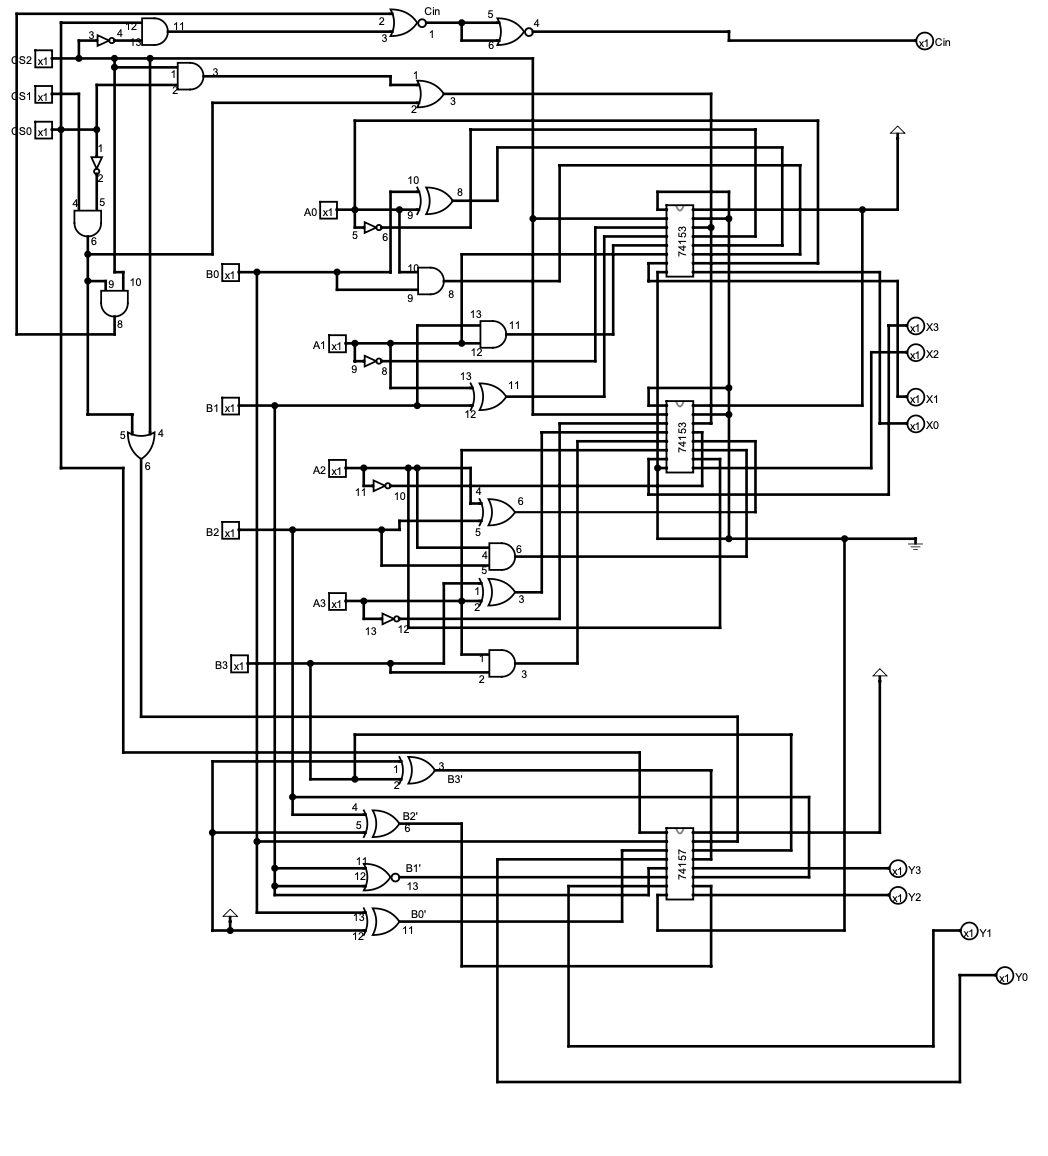
\includegraphics[width=1\textwidth]{Images/xiyi.png}
         \caption{$X_i$ and $Y_i$ circuit}
         \label{fig:xiyi}
     \end{figure}
     \begin{figure}[H]
         \centering
         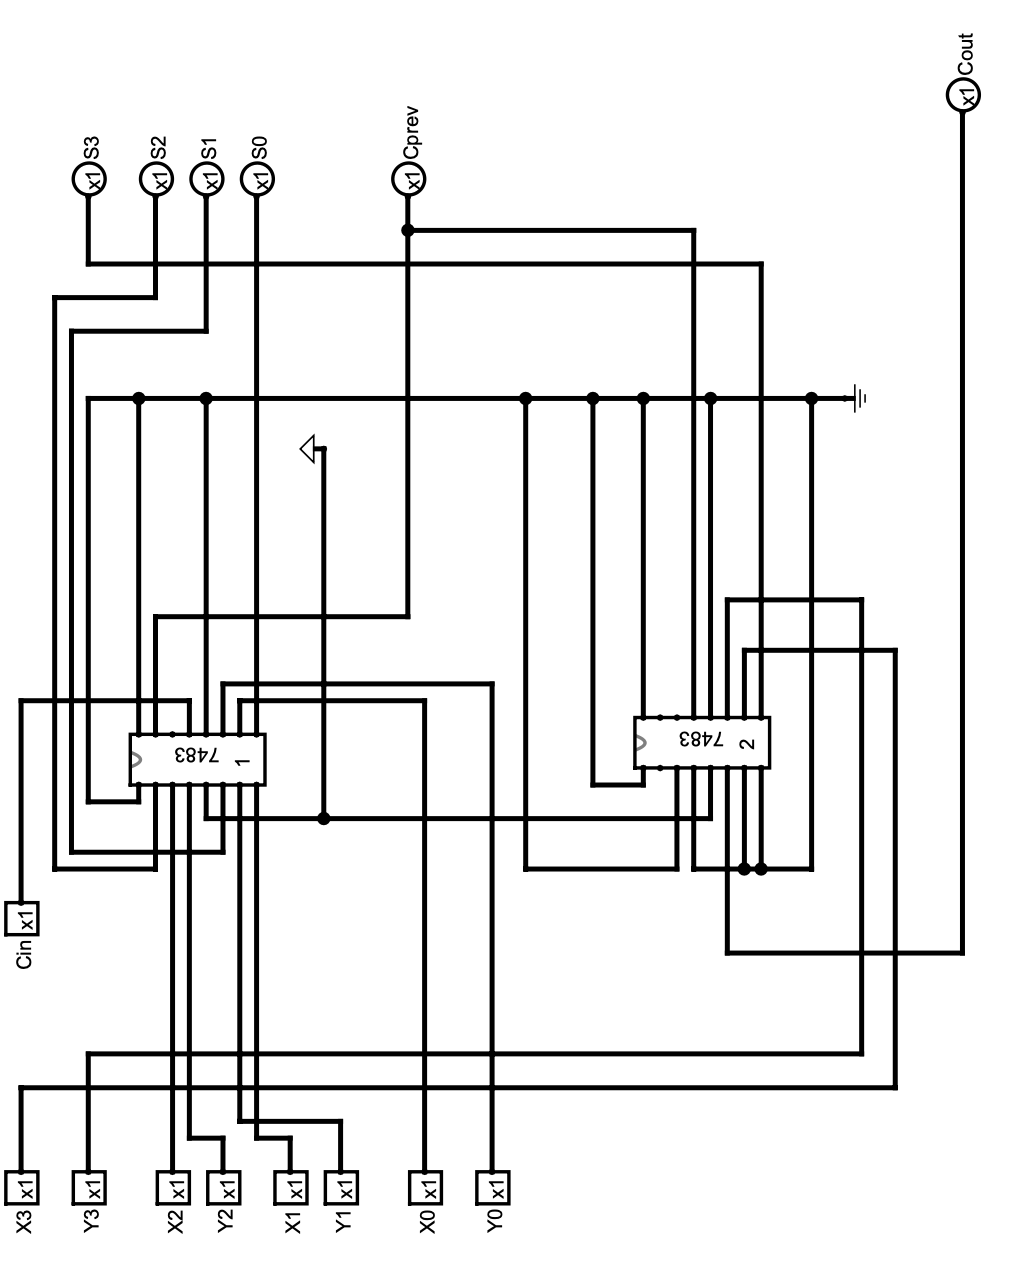
\includegraphics[width=0.8\textwidth]{Images/ModALU.png}
         \caption{Modified Two Adder ALU System}
         \label{fig:mod_alu}
     \end{figure}
     \begin{figure}[H]
         \centering
         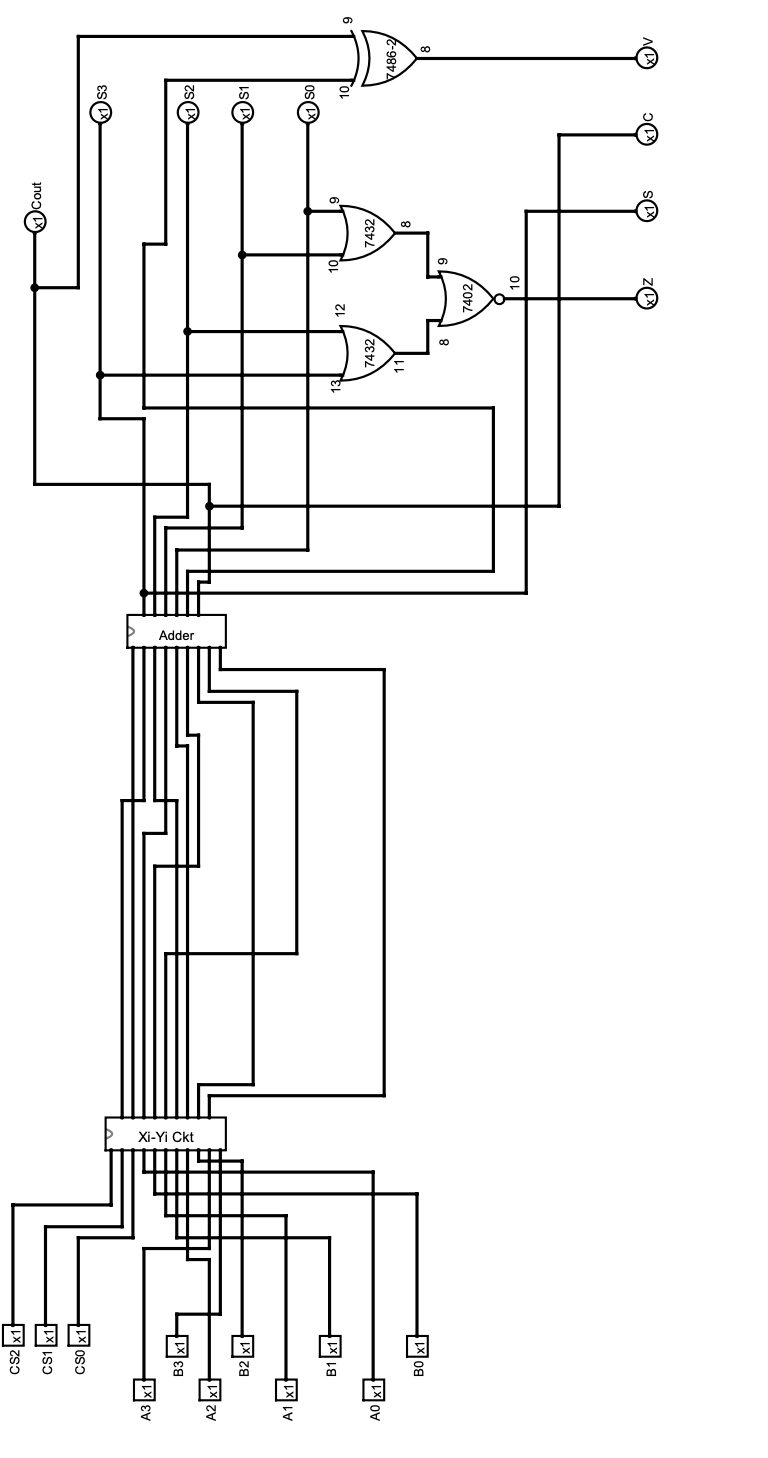
\includegraphics[height=20cm]{Images/ALU.png}
         \caption{Arithmetic and Logical Unit}
         \label{fig:alu}
     \end{figure}
     
     


\begin{figure}[H]
    \centering
    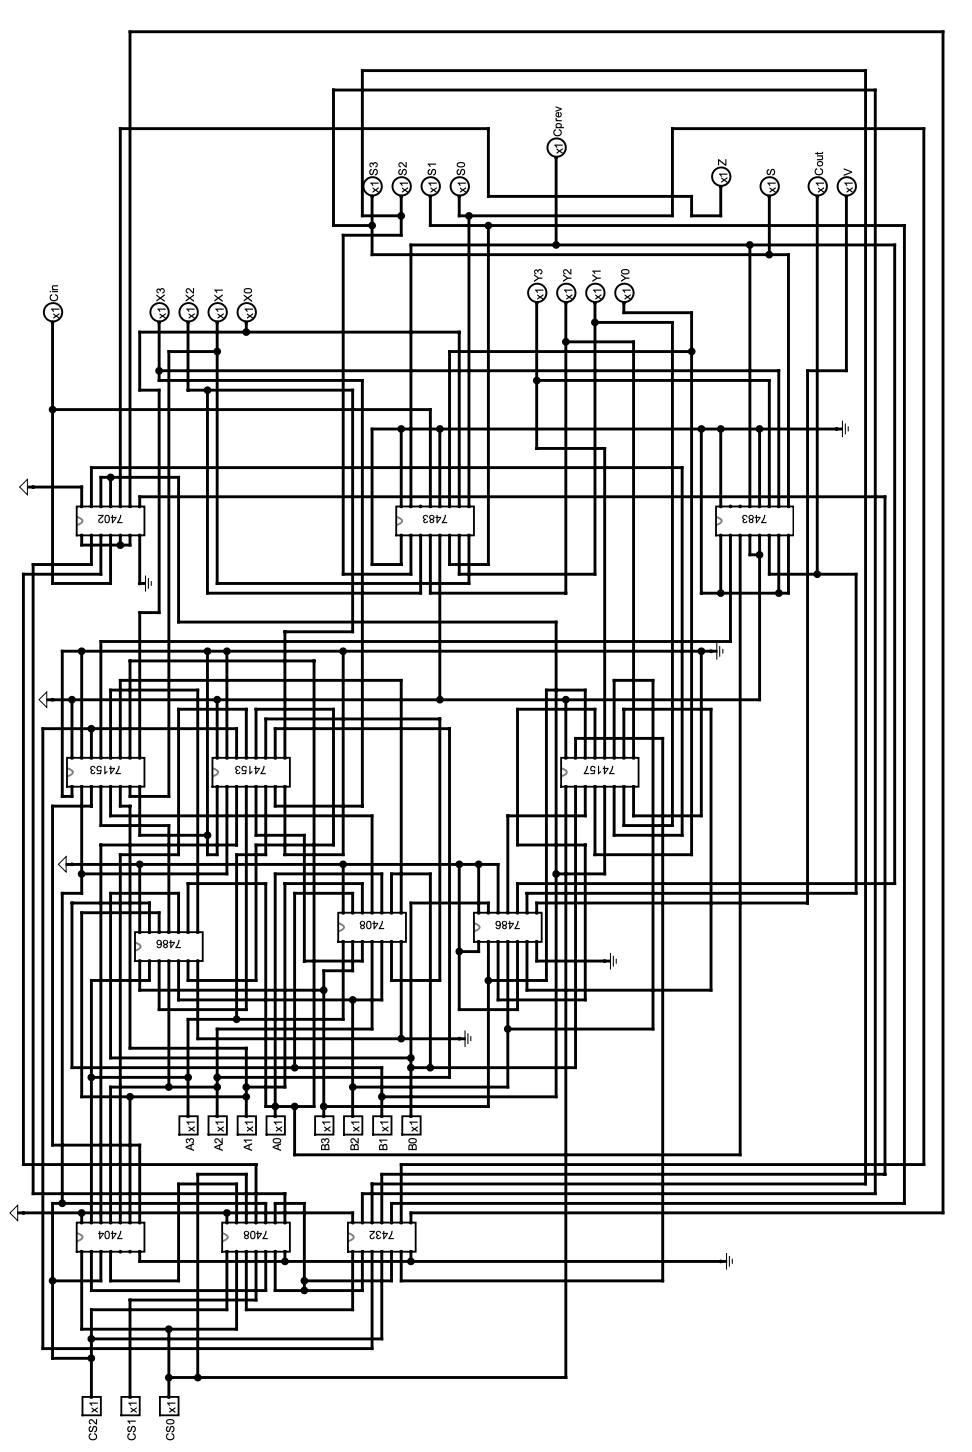
\includegraphics[width=0.8\textwidth]{Images/Combined.png}
    \caption{The Complete Design}
    \label{fig:comb}
\end{figure}

\newpage
\section{\large{ICs Used with Count as a Chart}}
\begin{table}[H]
    \centering
    \begin{tabular}{lc}
         \textbf{IC} & \textbf{Quantity}  \\
         \hline
         \hline
         IC 7402 & 1  \\
         IC 7404 & 1  \\
         IC 7408 & 2  \\
         IC 7432 & 1  \\
         IC 7483 & 2  \\
         IC 7486 & 2  \\
         IC 74153 & 2  \\
         IC 74157 & 1  \\
         \hline
         Total & 12  \\
    \end{tabular}
    \caption{ICs Used with Quantity}
    \label{tab:ic_quantity}
\end{table}



\section{\large{The Simulator Used along with the Version Number}}
Logisim - 2.7.1

\newpage

\section{\large{Discussion}}

In this assignment, we were tasked with implementing a $4$-bit ALU capable of performing $3$ arithmetic and $3$ logical operations.

\subsection{Design Finalization}

Initially, we had two designs, both requiring a similar number of ICs (13). The key difference was that one design used the adder for the XOR operation while handling the internal carry effectively. However, we ultimately chose the alternative design, which used two adders and a separate IC for the XOR operation. The reason for this choice was that both designs required the same number of ICs, but the latter was simpler to implement and understand. Additionally, in the final design, we had two free XOR terminals on the adder inputs, which we used for extra NOT operations, eliminating the need for an additional IC. We also cross-checked each K-map, noting that the negation of certain functions produced common terms, which could have been leveraged to reduce the number of ICs.

\subsection{Optimization}

Through extensive analysis, we worked diligently to minimize the number of ICs used. At one point, we realized that we were about to introduce a whole 7404 IC just for a single NOT operation. Instead, we opted to use a 7402 IC (\textit{NOR gate}). Initially, our design required 13 ICs, but we noticed that only two terminals of the 7432 (OR gate) were being utilized. By using two NOR gates, we replicated the OR function, and with another NOR gate, we handled the NOT operation. One actual NOR operation was required for the ZF flag, which would otherwise have consumed an OR and a NOT gate. Using the 7402, we managed to simplify this operation into a single IC. As a result, we removed the 7432 and 7404 ICs, replacing them with a single 7402 IC. Additionally, some NOT operations were handled using unused terminals on the 7486 (XOR gate). Further optimizations were made during debugging, which we discuss later.

\subsection{Hardware Implementation}

The hardware implementation posed significant challenges, including planning the placement of different components, minimizing wire lengths, and managing bulbs and switches. To maintain a clean hardware layout, we carefully routed wires to minimize crossing and ensure connections were as short as possible. Before powering up the ICs, we checked the voltage on each terminal to avoid damaging the ICs. We also verified the output at each stage before moving on to the next one. As one of the first groups to attempt the hardware implementation, we faced unique challenges. Our initial design failed because we couldn’t resolve a bug with one bit of $Y_i$, which forced us to redesign the ALU from scratch. Despite being more cautious, the second circuit still had several bugs.

\subsection{Debugging the ALU}

The new ALU design had a bug in the $X_1$ input. One of the NOT gates (terminals 5 and 6) was not producing the correct output. We were attempting to obtain $\overline{A_1}$ from $A_1$, but for some reason, it was malfunctioning, lighting up even when $A_1$ was \textit{ON}. Changing the IC didn’t fix the issue, and it was late at night, so we couldn’t go out to get a replacement NOT gate. We remembered, however, that we had some unused XOR gates in the second adder (IC 7483). We then managed to obtain $\overline{A_1}$ using the $S_3$ terminal of the second adder.

On the first day, we also encountered numerous issues with bulbs and switches. The switches didn’t fit properly in the breadboard, and we had to modify the pins. Eventually, we switched to a different type of switch that fit without issues. Furthermore, several bulbs were wasted because we didn’t initially realize that they had specific voltage and current thresholds.

\subsection{Conclusion}

Finally, after hours of hard work and troubleshooting, the ALU worked perfectly. The sense of accomplishment was surreal, and we successfully implemented the $4$-bit Arithmetic and Logic Unit (ALU) with the minimum number of ICs.


\section{Contributions}

\subsection{Software Implementation:}
\begin{itemize}
    \item \textbf{Design:} 2105047, 2405049, 2105046
    \item \textbf{Optimization:} 2105046
    \item \textbf{Logisim Simulation:} 2105047, 2105049
    \item \textbf{Verifying:} 2105055, 2105043
\end{itemize}
\subsection{Hardware Implementation:}
\begin{itemize}
    \item \textbf{Power and Ground:} 2105043, 2105049, 2105055
    \item \textbf{Pin Number Tracking:} 2105043, 2105047
    \item \textbf{Wire Management:} 2105043, 2105049
    \item \textbf{Wire Placement:} 2105046, 2105049, 2105055
    \item \textbf{Input:} 2105046, 2105049, 2105055
    \item \textbf{Verification:} 2105043, 2105047, 2105046, 2105055
    \item \textbf{Debugging:} 2105043, 2105046, 2105047, 2105049, 2105055
\end{itemize}
\subsection{Report:}
\begin{itemize}
    \item \textbf{Report Documentation:} 2105046
    \item \textbf{Complete Circuit Diagram:} 2105047
    \item \textbf{Block Diagram: } 2105055
\end{itemize}




\end{document}
